%\documentclass[fleqn]{book}
\documentclass[11pt]{amsbook}

\usepackage[turkish]{babel}

%\usepackage{../HBSuerDemir}	% ------------------------
\usepackage{../Ceyhun}	% ------------------------
\usepackage{../amsTurkish}


\begin{document}
% ++++++++++++++++++++++++++++++++++++++
\hPage{100}
% ++++++++++++++++++++++++++++++++++++++

    c) İ(1,3), Ç nin irgitilmiş altçizgesi değildir ve eğer iki \textit{tek üçgene} ortak bir ayrıt varsa, bunların düğümlerinin irgittiği altçizde D(4) dür,\\
    ç) Şekil 2.7.2 de gösterilen çizgelerden hiçbiri, Ç nin irgitilmiş altçizgesi değildir.


	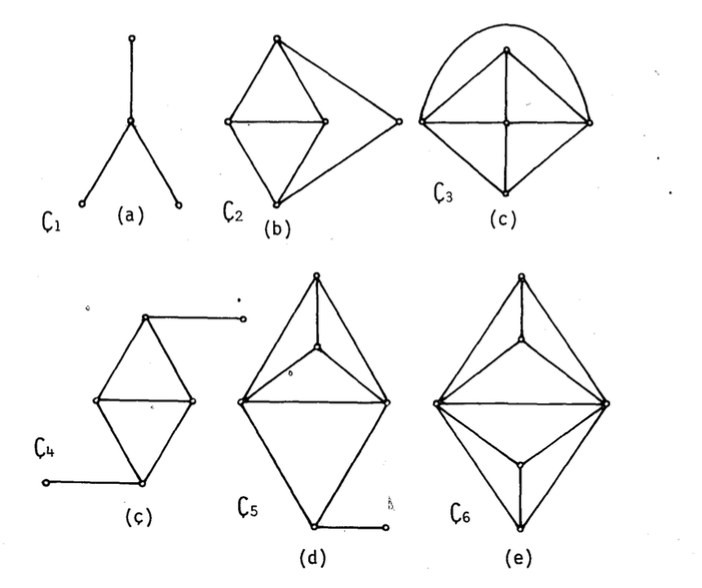
\includegraphics{images/ceyhunPage100}

\end{document}